\documentclass[review,3p,times,authoryear,12pt]{elsarticle}
\usepackage{amsmath,amsthm,amssymb}
\usepackage{algorithm}
\usepackage{graphicx,subfigure}
\usepackage{clrscode3e}
\usepackage{enumerate}
\graphicspath{{figure/}}
\newtheorem{proposition}{Proposition}

\begin{document}
\begin{frontmatter}
\newpage

\title{The Stowage Stack Minimization Problem with K-Rehandle Constraint}
\author[shu]{Ning Wang}
\ead{ningwang@shu.edu.cn}

\author[shu]{Shanhui Ke}

\author[syu]{Zizhen Zhang\corref{corl}}
\ead{zhangzizhen@gmail.com}

\address[shu]{
Department of Information Management, School of Management, Shanghai University, Shanghai, China
}
\address[syu]{
School of Data and Computer Science, Sun Yat-Sen University, China
}
\cortext[corl]{Corresponding author. Fax: +852 ********, Phone: +852 ********}

\begin{abstract}
The Stowage Stack Minimization Problem (SSMP) investigates a stowage planning problem when carriers have the obligation to ship all the given containers in different ports, with the objective to utilize the fewest number of stacks on the ship. This problem has realistic usefulness since it can help shipping forwarders estimate shipping space of each shippers.
To our best knowledge, we propose SSMP for the first time in the academic community.

In this paper, we talk about SSMP with K rehandles (SSMP-KR). A heuristic algorithm is put forward to construct solutions to the SSMP-KR. We discuss the theoretical performance guarantee of the algorithm using mathematical inequations and induction.
To evaluate the actual performance of our algorithm, we conduct experiments on a set of instances with practical size and compare the results when different values of K are selected.
What's more, instances with different values of ports, containers and heights have been tested to make sure the universality of our algorithm.
\end{abstract}

\begin{keyword}
Containership stowage planning\sep stack minimization \sep K-rehandles \sep constructive heuristic
\end{keyword}
\end{frontmatter}


\section{Introduction}
\label{sec:i}
International trade plays an important role in promoting the development of world economy.
Maritime transport is the backbone of globalization and lies at the heart of cross-border transport networks that support supply chains and enable international trade.
Nowadays, over 80\% of world trade is carried by the maritime freight industry, which operates the container transportation business \citep{zhang2016multiobjective}.
In 2015, world seaborne trade volumes surpassed 10 billion tons shown in ~\cite{unctad2016}.

Container-shipping is a kind of modern transportation tool which has a lot of advantages in speed, security, and quality comparing with the break-bulk cargo ship.
Containerization is an important driver of the global economy, and the container has become a mainstay of worldwide trade.
According to World Shipping Council, around 52\% of the value of world international seaborne trade today is being moved in containers.
This mode is deeply accepted by shippers and carriers, and is becoming the main trend of freightage in the world.
It has resulted in a tremendous growth of the maritime freight industry and it shows powerful vitality and promising prospects.

With the development of container-shipping, more and more containers are transported by sail.
Over the past decades there has been a continuous increase in demand for cost efficient containerized transportation.
Thus, it makes higher research demand.
The container stowage plan is a pivotal link to containers transportation, and the objective of which is to draw a plan of loading and discharging sequence of containers for containership in \cite{zhang2008review}.
The most frequently used addressing notation for storage locations in a container ship is the bay-row-tier system.
The cargo space of a container ship is split into several 20-ft-long areas. 
These areas are termed as 20-ft bays (see Figure \ref{fig 1:graph}).
\begin{figure}[htbp]
\center
\resizebox{0.5\textwidth}{!}{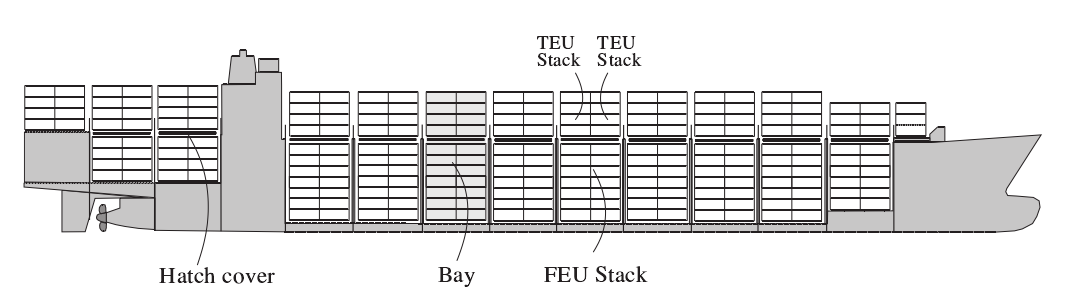
\includegraphics{figure/Arrangement_of_cargo_space.png}}
\caption{The arrangement of cargo space in a container vessel.}
\label{fig 1:graph}
\end{figure}

In addition, two contiguous 20-ft bays form a 40-ft bay which can be used to accommodate 40-ft containers.
Each bay consists of container stacks placed along the width of ship.
Container stacks in a bay are indexed by a row number.
All bays are divided into an over deck and an deck area, separated by structures called hatches.
The container position in the ship is uniquely indexed by (bay, row, tier).
Such three-tuple is called a slot.
However, slot in this paper is indexed by (stack, tier) for the sake of research convenience.
On the under deck, the parts of a bay are divided into stacks/slots that are one container wide, and are composed of two Twenty-foot Equivalent Unit (TEU)
stacks and a single Forty-foot Equivalent Unit (FEU) stack (see Figure \ref{fig 2:graph}).
In our paper, we assume that all the containers are of the same size, (e.g. 20 TEUs) and each slot can be fully occupied by one container.





\begin{figure}[htbp]
\center
\caption{a front view of a vessel bay.}
\resizebox{0.5\textwidth}{!}{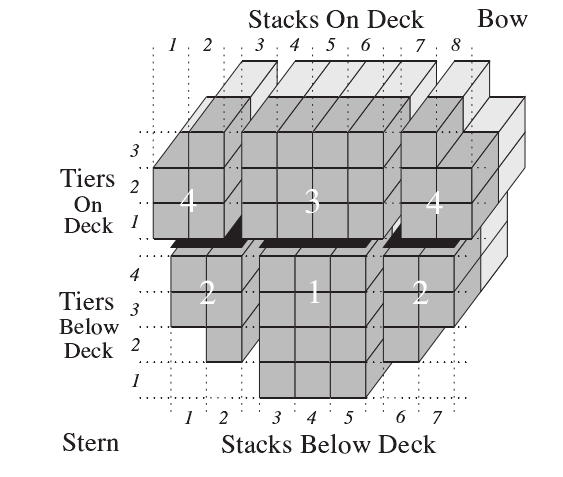
\includegraphics{figure/A_vessel_bay.png}}
\label{fig 2:graph}
\end{figure}

Each container has a weight, height, length and port where it has to be loaded (origin port) and unloaded (destination port).
Unloading and loading movements of same containers in the same port are called rehandles.
Rehandles arise either when we want to unload containers destined for current port which however are beneath those destined for subsequent ports, or when we want to reorder the sequence of containers to prevent more rehandles in the future.
Usually it is called necessary rehandles in the former case and voluntary rehandles in the latter.


TODO: why rehandles exists.
Actual examples show that containership stowage plans not only influence the income of shipping company from transportation but also have direct relation to the safety of ships and freights.
The problems have troubled and aroused the interests of both scholars and commercial shipping organization in many countries since 1970s~\citep{webster1970container}.
The previous research ignores the importance of the capacity of ship and give much emphasis on the balance of ship, the number of rehandle and so on.
Nevertheless, we ought to think about the importance of capacity as well.
For example, if we use each stack sufficiently, the required number of ships will be reduced and thus the cost decreases.
The problem mentioned in this paper gives a priority on how to reduce the number of used stacks with $K$ rehandles.
On one hand another aspect of container stowage planning is exhibited through the research on this problem and the shipping cost can be reduced by using the heuristic algorithm that we propose in this paper.
On the other hand, it represents a novel thinking perspective to make research about the problem and it will promote the development of shipping optimal problem.

We put forward the stowage stack minimization problem with $K$ rehandles constraint problem (SSMP-KR) in this paper.
Literally speaking, it is a container stowage planning problem whose objection is to figure out the minimization of used stacks with $K$ rehandles constraint on a given container shipping.
The heuristic algorithm in this paper uses the greedy rule to decide the loading and unloading operations for each container to be loaded and unloaded in each port along the voyage.
Therefore, the solution we get is the approximately optimal rather than the global optimal.

%TODO: The contribution of our paper lies in three aspects. First, Second, Third.
The contribution of our paper lies in three aspects.
First, the previous research usually focused on how to reduce the rehandles or shifts, our paper initially considers how to get the optimal container stowage plan when giving the number of allowed rehandles.
Second, the problem can also be regarded as a extended problem of the stowage stack minimization problem with zero rehandle, which is a combinatorial optimization problem.
Furthermore, we can get the different results when the values of $K$ are different. In addition, each instance with zero rehandle can be a benchmark instance.
Instances only have the different values of $K$ can compare with their benchmark instances to get some conclusions we need.
By comparing different results, we eventually choose a appropriate value of K to balance the complexity of quay operations and the space utilization of the cabin.
Third, we put forward a heuristic algorithm to solve the problem proposed in this paper and the results show the good performance of our algorithm.
The results can help us know the stowage plan visibly and make analysis about what the appropriate $K$ is.
Therefore, the problem and the algorithm presented in our paper are both novel and worthy of further study.


The remainder of this paper is organized as follows: we review extant research works in Section~\ref{sec:lr} and the formal definition of our problem and its some properties are provided in Section~\ref{sec:pd}.
In Section~\ref{sec:algo} we present our heuristic algorithm for the problem, as well as explain the ideas  and specific details about the algorithm.
Experiments and associated analysis are illustrated in Section~\ref{sec:ea}. Concluding remarks close the paper in Section~\ref{sec:con}.

\section{Literature Review}
\label{sec:lr}
The container stowage problem can be divided into two classes: one is management and programming at the container terminal, the other is stowage plan for containership.
This paper mainly focuses on the latter.
Sorted by research method, this problem will be divided into six categories: simulation based on  probability, heuristic procedures, mathematical programming approach, decision support system, expert system and evolutionary computation.
The following are some reviews about these categories of containership stowage plan.

Since 1970s, the stowage plan problem has been studied by shipping organization for commercial demand.
They tried to find a good solution which would satisfy fewer shifting and higher efficiency when loading and discharging containers.

\cite{shields1984containership} introduced a computer preplanning system (CAPS) which had been used by American President Lines.
The CAPS produced stowage plan by using Monte Carlo theory.
\cite{dillingham1986application} introduced their researches on expert system of stowage based on rules.
Each of the suggested container movements was displayed graphically as the decisions were made.
\cite{wilson2001container} outlined a computer system that generated good sub-optimal solutions to the stowage pre-planning problem.
The methodology progressively refined the arrangement of containers within the cargo-space of a container ship until each container is specifically allocated to a stowage location.

\cite{scott1978loading} constructed a model, in which containers were sorted into ten classes based on some characteristics and then three heuristic rules were used to assign gradually each type of containers to slots of the ship by four steps, while the shifting problem had not been considered in their model.
\cite{avriel1998stowage} presented a 0-1 binary linear programming formulation based on minimizing the number shifting in a single bay of a ship calling at a given number of ports.
Further, they showed that finding the minimum number of columns for which there was a zero shifts stowage plan is equivalent to finding the coloring number of circle graphs.
\cite{botter1991stowage} created a model called complete mathematical model for the stowage plan problem, which used binary decision variables to determine the containers unloading and loading sequence for each port.
However, literatures have shown that binary linear programming formulation for such problems is impracticable for real life problems due to the large number of binary variables and constraints.

\cite{avriel1998stowage} and \cite{avriel2000container} focused on stowage planning in order to minimize the number of unproductive shifts (temporary unloading and reloading of containers at a port before their destination ports in order to access containers below them for unloading).
A binary linear programming (LP) model was formulated without considering ship's stability and other real-life constraints.
Due to the proven NP-hardness of the problem, a so-called "Suspensory Heuristic" --- based on earlier work by \cite{avriel1993exact} --- was developed in order to solve even large problem instances.
The heuristic assigned slots in a bay to containers dynamically with respect to the sequence of ports in a vessel's route.
\cite{haghani2001model} proposed a MIP model for developing loading plans in order to minimize the time that a vessel spent at port, and the container handling cost which shifts caused by was highly influenced by the number of unproductive but necessary an unsatisfactory arrangement of containers.
In \cite{ambrosino2004stowing} the problem of stowing containers into a containership had been faced by evaluating an exact 0-1 Linear Programming model, which was not practically useful for large cases.
This had been modified by an approach proposed by the authors, consisting of heuristic preprocessing and prestowing procedures that also allow the relaxation of some constraints of the exact model.
The proposed approach exhibited very good performance in terms of both solution precision and computational time.
Moreover, in the performance evaluation with real size cases, it also guaranteed another very important maritime performance index, in term of handling operations/hour.
In \cite{Delgado2012251}, they focused on the slot planning phase and presented a Constraint Programming and Integer Programming model for stowing a set of containers in a single bay section.
This so-called slot planning problem was NP-hard and often involved stowing several hundred containers.
Using state-of-the-art constraint solvers and modeling techniques, however, they were able to solve 90\% of 236 real instances from our industrial collaborator to optimality within 1 second.
\cite{ambrosino2015mip}  proposed a Mixed  Integer  Programming (MIP) heuristic aimed at determining stowage plans in circular routes for container ships so as to give support for the ship coordinator and the terminal planner.



\cite{webster1970container} first tried to solve the problem by using computer. They put forward a heuristic algorithm that could create a random stowage plan.
What's more, \cite{ding2015stowage} developed a heuristic algorithm which can generate stowage plans with a reasonable number of shifts for such problems.
The algorithm, verified by extensive computational experimentations, performed better than the Suspensory Heuristic Procedure (SH algorithm) in \cite{avriel1998stowage}, which was a dynamic slot-assignment scheme that terminated with a stowage plan, and to the best of our knowledge, is one of the leading heuristic algorithms for such stowage planning problem when there are many binary variables and constraints in the formulation.

Tabu search was employed to obtain an optimal solution in \cite{wilson2001container} and his model was feasible because it can change configuration step by step until each container was assigned to specific slot.
Then, \cite{bortfeldt2003parallel} presented a parallel tabu search algorithm for the container loading problem with a single container to be loaded.
According to an extensive comparative test also including heuristics from other authors, high utilizations of the container volume are already obtained with the sequential TSA (tabu search algorithm).
A slight improvement of these results could be achieved by the parallelization.
The Ship Stowage Planning Problem had been addressed in \cite{Monaco2014256}.
They first provided a detailed description of the two phases in which the decision problem is usually decomposed, along with a classification scheme and a review of the most relevant related papers.
They proposed a Binary Integer Model for the minimization of the transportation times of the containers and the yard-shifts and they developed a Tabu Search Algorithm for finding sub-optimal solutions to the problem and have solved the model by CPLEX.


Algorithm of evolutionary computation came from Darwin��s biologic theory of evolution. There are two or three branches at present, among which genetic algorithm is used widely.
The presented hybrid GA for loading a single container in \cite{bortfeldt2001hybrid} was particularly suitable for strongly heterogeneous containers stowage problems.
The algorithm took account of some constraints which were relevant in practice.
Its good performance and superiority to comparative methods had been verified in an extensive test.
The use of a time limit kept the required computing times within acceptable limits.
\cite{dubrovsky2002genetic}  used a GA for solving the stowage planning problem of minimizing the number of container movements.
Search space was significantly reduced by a compact and efficient encoding scheme.
Ship stability criteria were reflected by appropriate constraints.
Simulation runs demonstrated the efficiency and flexibility of the GA-based approach.
\cite{kammarti2013evolutionary} proposed an efficient genetic algorithm which consists on selecting two chromosomes (parent) from an initially constructed population using a roulette wheel technique.
Then, the two parents were combined using a one point crossover operator.
Finally, a mutation operator was performed.
The variant tackled in \cite{cohen2017container} involved several constraints, inspired by real-life problems and application found in the literature.
Given the complexity of the problem, which belongs to the class of NP-hard problems, a novel evolutionary metaheuristic algorithm is developed and designed.
Considering the ability and flexibility of Genetic Algorithm (GA), the approach was based on a two-phase procedure, one for master planning and the other for allocation of the containers into slots.
GA parameters were analyzed to achieve practical and best results.
The system offered stowage allocation solutions for both phases, thus offering flexibility for a wide variety of vessels and route combinations.

Container ship stowage problem(CSSP) is combinatorial optimization problem with multiobjects and multiconstraints.
In order to reduce computational difficulty, CSSP was decomposed two subproblems in \cite{wei2005model}, and the first one was discussed detailed.
CSSP was regarded as bin-packing problem.
After being modeled��the algorithm of best fit for binpacking problem was used to solve the CSSP.
A case showed that the algorithm was feasible for container ship stowage problem.
A multiobjective ship stowage planning problem(SSPP) was investigated by \cite{zhang2016multiobjective}, which aimed to optimize the ship stability and the number of rehandles simultaneously.
They used metacentric height, list value, and trim value to measure the ship stability.
Meanwhile, the number of rehandles was the sum of rehandles by yard cranes and quay cranes and all necessary rehandles at future ports.
The algorithm could produce a set of nondominated solutions.
Decision makers could then choose the most promising solution for practical implementation based on their experience and preferences.
Extensive experiments were carried out on two groups of instances.
The computational results demonstrated the effectiveness of the proposed algorithm compared to the NSGA-II and random weighted genetic algorithms, especially when it was applied in solving the six-objective SSPP.

\cite{tierney2014complexity} investigated the complexity of stowage planning problem and showed that the capacitated k-shift problem is solvable in polynomial time for any choice of stacks and stack capacities.
Some scholars paid special attention to the process of loading and unloading, \cite{malucelli2008stack} investigated stack reordering strategies aiming at minimizing the number of pop and push operations and  focused on three versions of the problem in which reordering can take place in different phases: when unloading the stack, when loading it or in both phases.
There are some extended problems in this field.
Different problems arising in practice in the context of storage areas organized in stacks have been surveyed by \cite{Lehnfeld2014297}.
Different problem classes have been identified, namely loading, unloading, premarshalling and combined problems.
To be able to categorize all these problems in a more abstract way, they developed a classification scheme which had been used to summarize complexity results and solution methods for all problem classes.
In conclusion, many problems have already been solved by exact or heuristic methods in all four considered problem classes.
Nevertheless, due to the diversity of the problems, various other versions exist.
For further research, a major challenge is the development of more efficient solution algorithms integrating additional constraints coming from practical applications.
As we all known, the 3D Container ship Loading Plan Problem (CLPP) is an important problem that appears in seaport container terminal operations and is well known to be NP-hard.
This problem consists of determining how to organize the containers in a ship in order to minimize the number of movements necessary to load and unload the container ship and the instability of the ship in each port.
In \cite{Araujo201650},  the hybrid method Pareto Clustering Search (PCS) was proposed to solve the CLPP and obtain a good approximation to the Pareto Front.
The PCS aimed to combine metaheuristics and local search heuristics, and the intensification was performed only in promising regions.
Computational results considering instances available in the literature were presented to show that PCS provides better solutions for the CLPP than a mono-objective Simulated Annealing.

To the best of our knowledge, apart from the SSMP-ZR, only \cite{avriel2000container} and \cite{jensen2010complexity} discussed the stowage stack minimization and its connection with the chromatic number of circle graphs when the stack height is unlimited.
At present, the research tendency of the stowage planning problem is intelligent management system, which is a new stowage research direction.
Intelligent containership stowage plan system is a technological innovation in contrast with traditional stowage method.
It can improve the ability of decision-making management system of container shipping by means of artificial intelligence, information technology, communications and computer technology.


\section{Problem Description and properties}
\label{sec:pd}

A ship starts its journey at port 1 and sequentially visits port 2, 3, ..., $P$, 1, 2, 3, ... $P$, 1, ..., which forms a circular route.
There are standard containers to be shipped along the journey.
Some containers are shipped from $i$ to $j$ ($i<j$) and some containers are shipped from $i$ to $j$ ($i>j$) going across port 1.
Hence, it is easy to understand that containers with $O(i)<D(i)$ and with $O(i)>D(i)$ both exist.
Moreover, the ship is never empty once sets out due to the circular feature.

Supposing that the voyage terminates in the second circle, we can break the loop into a straight line.
A ship starts its journey at port 1 and sequentially visits port 2, 3, ..., $P$, 1, 2, 3, ... $P$.
There will be $P$ kinds of different containers according to their origin ports.
Containers at port 1 can be transported into port 2, 3, ..., $P-1$, $P$.
Containers at port 2 can be transported into port 3, 4, ..., $P$, 1.
The last kind of containers originates from port $P$ and can be transported into port 1, 2, ..., $P-1$.
However, we only work out the result under the condition that $O(i)<D(i)$ happens for the convenience of experiment design.
Consequently, we need break the loop voyage into the line voyage.
Actually it is not difficult, we can regard the port 1 in the second circle as port $P+1$, the next port in the second circle will be port $P+2$ and so on.
%It can be applied into the other circumstance when $O(i)>D(i)$ happens if we regard port $O(i)$ as the port 1 in the special circular route.
Eventually we only need work out the container stowage planning for the line voyage from port 1 to port $2P$ and it is equivalent to cope with the problem with a two-loop voyage.
Similarly, we can use this method to deal with the circular route container stowage problem no matter how many loops there are.
There is another approach we can figure out to solve the circular route problem.
After going across port 1 in each circle, we reset the origin port of containers remained in vessel as port 1.
For example, containers from port 3 to the port 2 in the next circle will be containers from 1 to port 2 after going across port 1 in the next circle.
Thus, it only exists the port from port 1 to port $P$.
In addition, all the loading and discharging ports of $N$ containers are known in advance.
That's to say, we adopt the so-called "look ahead"  mechanism, which can make use of all loading information available.
It is helpful for us to make detailed container stowage plan.

At each port, the containers destined to the current port are discharged, and the containers stowed at the port are loaded to the ship.
Each container $i$ is characterized by its shipping leg $O(i)\rightarrow D(i)$, indicating that the container is loaded at port $O(i)$ and discharged at port $D(i)$.
The containers remain unmoved when the ship voyages among the ports.
Rehandles may occur in these ports, either necessary or voluntary or both.
A container is called a j-container if it is destined for port j.
0bviously all j-containers are loaded before the ship visits port j and should be unloaded at port j.
A j-container is called a i, j-container if it is originated from port i.
A j-container in slot (s, t) is said to be blocked if there exists a j'-container in slot (s', t) with j' $>$ j and s'$<$s, and the j'-container is called a blocking container with respect to the j-container.
Occurrence of container blocking at any time means that shifts are no longer avoidable.

We assume that the ship has enough capacity to accommodate all the containers along the journey.
The ship spaces are divided into several stacks.
Each stack can hold at most $H$ vertically piled containers, i.e., the height limit of every stack is $H$.
When $H$ is bounded, we call the SSMP-KR as the Capacitated SSMP-KR (CSSMP-KR);
when $H$ is sufficiently large (e.g., $H\geq N$) or unbounded, we refer to it as the Uncapacitated SSMP-KR (USSMP-KR).
For the CSSMP-KR, if the number of containers in a non-empty stack is less than $H$, the stack is termed as a \textit{partial} stack;
otherwise it is a \textit{full} stack.
The objective of the SSMP-KR is to transport all the containers using the fewest number of stacks with K rehandles allowed.
The USSMP-KR is far from the real situation in the stowage planning, since stack heights of ships are restricted by operation cranes.
Hence, this paper give emphasis on the CSSMP-KR and for the convenience of description, we use SSMP-KR for short in this paper.

A feasible solution to the SSMP-KR with the container stowage plan is represented by a operation set, from which we can clearly know the slot changing of each container, even when there is an overstowage.
We have also given the layout of containers in vessel after loading and unloading each container to help us observe the result.
The detailed introduction will be given in the following section.

Considering that the complexity of working out the integer model for the SSMP-KR problem, we give the IP model for the capacitated SSMP-ZR problem for reference.
The capacitated SSMP-ZR can be mathematically formulated by the following integer programming (IP) model.

\begin{small}
\begin{align}
& (IP)~~\min\hspace{6pt}\sum_{s=1}^{S} y_s \label{eqn:obj} \\
& \mathrm{s.t.}\hspace{11pt}\sum_{s=1}^{S} x_{is}=1, ~\forall 1\le i \le N \label{eqn:1}\\
%\mbox{s.t.~}& \sum_{c=1}^{C} x_{ic}=1, ~\forall 1\le i \le m \label{eqn:1}\\
& \hspace{24pt}\sum_{i=1}^{N} x_{is}\le M y_s, ~\forall 1\le s \le S	\label{eqn:2}\\
& \hspace{2pt}\sum_{i:O(i)\le p\le D(i)-1} x_{is}\le H, ~\forall 1\le s\le S, 1\le p\le P		\label{eqn:3}\\
& x_{is}+x_{js}\le 1, ~\forall 1\le s\le S, 1\le i,j\le N, O(j)<O(i)<D(j)<D(i)	\label{eqn:4}\\
& x_{is}, y_s \in \{0,1\}, ~\forall 1\le s\le S,1\le i,j\le N
\end{align}
\end{small}

In the above model, $M$ is a sufficiently large number and $S$ is the number of stacks on the ship.
$x_{is}$ is a binary decision variable which is equal to 1 if container $i$ is loaded to stack $s$, and 0 otherwise.
$y_s$ is a binary decision variable that is equal to 1 if stack $s$ is used for stowage, and 0 otherwise.
$O(i)$ and $D(i)$ indicate the shipping leg of container $i$. The objective (\ref{eqn:obj}) minimizes the number of stacks used.
Constraints (\ref{eqn:1}) ensure that each container $i$ is loaded to only one stack.
Constraints (\ref{eqn:2}) guarantee that containers can only be loaded to used stacks.
Constraints (\ref{eqn:3}) assure that at each port $p$, the number of containers in stack $s$ does not exceed $H$.
Constraints (\ref{eqn:4}) avoid overstowage requiring that container $i$ is prohibited to block container $j$ in the same stack when container $j$ is retrieved.

It is straightforward that the resultant layout from such a loading order does not include overstowage.

We have also presented the simple IP model for the SSMP-KR to make our problem clear.
The SSMP-KR can be mathematically formulated by the following integer programming (IP) model.

\begin{small}
\begin{align}
            & (IP)~~\min\hspace{6pt}\sum_{s=1}^{S} y_s \label{eqn:obj2} \\
\mbox{s.t.~}&\sum_{s=1}^{S} x_{is}=1, ~\forall 1\le i \le N \label{eqn:5}\\
            &\sum_{i=1}^{P} R_i \le K \label{eqn:6}\\
            &\sum_{i=1}^{N} x_{is}\le H, ~\forall 1\le s \le S	\label{eqn:7}\\
            & ~~\max\hspace{6pt}\sum_{i=1}^{P} (L_i-U_i+R_i) \le S*H \label{eqn:8}
\end{align}
\end{small}

In the above model, $H$ is the limit height of each stack, $N$ is the number of containers, $P$ is the number of ports and $S$ is the number of stacks in the vessel.
$x_{is}$ and $y_s$ have the same notations as the IP model for SSMP-ZR.
$L_i$, $U_i$, $R_i$ are the number of loading containers, discharging containers and rehandling containers, respectively.
The objective (\ref{eqn:obj2}) minimizes the number of stacks used.
Constraints (\ref{eqn:5}) ensure that each container $i$ is loaded to only one stack.
Constraints (\ref{eqn:6}) guarantee that the total number of rehandles is no greater than than $K$, the value of allowed rehandles.
Constraints (\ref{eqn:7}) ensure that the total number of containers in each stack is no greater than than $H$.
Constraints (\ref{eqn:8}) assure that at each port $p$, the number of containers in vessel does not exceed $S*H$.

Note that the solution to the IP model only reflects the assignment of containers to stacks.
It can be converted to a complete loading plan as follows.
At each port $p$, load containers to their corresponding stacks (given by $x_{is}$) by the decreasing order of their destinations.
Comparing with the IP model for the capacitated SSMP-ZR, we can find that the resultant layout from such a problem model will be more flexible to design our algorithm and closer to the actual situation.

\section{Methodology}
\label{sec:algo}
In this section, we will talk about the heuristic algorithms to the SSMP-KR as well as the basic performance guarantee of the algorithms.

\subsection{Heuristic Algorithms for the SSMP-KR}
\label{sec:h1}

Before the introduction of our algorithm, we give the related notations as followings in Table \ref{tab:1}:

\begin{table}[htbp]
\scriptsize
  \centering
  \caption{constants, sets, variables and methods in the algorithm}
    \begin{tabular}{r|l}
    \hline
     $K$, $P$ ,$N$ , $H$ & the meanings of these constants are the same as what described in the above\\
     $LB$ & the lower bound for each given instance\\
     $UB$ & the upper bound for each given instance\\
     $S_0$ & stack index set to store feasible stacks when there isn't an rehandle allowed\\
     $S_1$ & stack index set to store partial stacks without rehandles when $K$ doesn't reach\\
     $S_2$ & stack index set to store partial stacks with rehandles when $K$ doesn't reach\\
     $S_3$ & stack index set to store empty stacks when $K$ doesn't reach\\
     $height$ & a one-dimension array, represents the current height of each stack\\
     $Layout$ & a two-dimension array, represents the layout of containers in vessel after each operation\\
     $Numofstack$ & the cumulative number of used stacks\\
     $nearport$ & a one-dimension array to store the nearest port in all containers for each stack\\
     $lb$  & a one-dimension array, represents the lower bound of used stacks in each port\\
     $ub$ & a one-dimension array, represents the upper bound of used stacks in each port\\
     $ac$ & an arraylist to ordinally store the information of each container including the origin port and the destination port\\
     $Solution$ & an arraylist to ordinally store the operation of each container\\
     $Container$ & a Class to record the information of each container\\
     $Operation$ & a Class to record the information of each operation, including loading, unloading and rehandling\\
     $heuristic()$ & the main method to complete the container stowage planning along the voyage\\
     $read()$ &  a method to read the parameters and the detailed containership information from each instance\\
     $bound()$ & a method to provide a lower bound and upper bound and can be used to prove our algorithm's rationality\\
     $GetstackNum$ & a method to get the sequence number of chosen stack\\
   \end{tabular}
   \label{tab:1}
\end{table}



If the allowed K doesn't reach When loading containers, we use arraylist $S_1$ to store partial stacks without rehandles occuring, arraylist $S_2$ to store partial stacks with rehandles occuring, arraylist $S_3$ to store empty stacks.
The priority order of them is $S_1$, $S_2$, $S_3$.
If there isn't an overstowage allowed when loading containers, we use $S_0$ to store the feasible stacks.
For ease of illustration, we need to explain the definition of nearport.
For example, three containers are stored in the same stack, and their destination ports are 4,5,6, respectively, then the value of nearport of this stack is 4.
If a stack is empty, its nearport will be set to $P+1$, here $P$ is the total number of the ports along the voyage.

For the sake of description, we will use some notations presented in Table \ref{tab:1}.
We firstly talk about the simple condition that the allowed rehandles run out.
When traversing all the stacks to choose the optimal one for each container according to our rules, we add non-full stacks whose nearest port is no smaller than the current loading container into arraylist $S_0$.
For the stacks in $S_0$, we choose the one with the nearest port.
Afterwards, we talk about the complex condition that the rehandles are allowed.
Undoubtedly, it is a little different from the simple condition.
Under this condition, $S_1$ have the highest priority.
If $S_1$ is null, we choose the stack from arraylist $S_2$ which is used to store partial stacks whose nearest port is smaller than the current loading container.
Both in $S_1$ and $S_2$, we choose the stack whose nearest port is smallest.
If $S_2$ is null, we choose the first stack when we traverse the $S_3$ which is used to store empty stacks.
So it is the loading rules in the above and the following is the discharging rules.

When discharging containers, we just need to unload containers from top to bottom one by one when the container's destination port is the current port if there isn't an overstowage in the stacks.
when overstowage happen, we have to unload the blocking containers before discharging those right containers.
As for blocking containers, we will reset their origin ports as current port after unloading them and their destination ports remain unchanged.
That's to say, the outbound containers at the current port increase.

We give out some key procedures of our algorithms in the following context:
For all the ports along the voyage, we adopt the heuristic method to dispose for the given input.
Through the heuristic method, we can transfer the input into the output.

The following pseudo gives a simplistic explanation of heuristic method, which is our main method.

\begin{algorithm}
  \caption{The procedure of the heuristic() method}
  \label{alg:1}
  \begin{codebox}
  \Procname{\proc{Heuristic() method for the SSMP-KR}}

    \li \For each port $p=1, 2 , \ldots,P $.
     \li \Do
                Unload containers destined at port $p$.

                Load containers originated from port $p$.
    \li   \For each stack $i=1, 2, \ldots, UB$.
    \li \Do
              work out the value of Numofstack through counting the number of non-empty stacks.
          \End
       \End
\end{codebox}
\end{algorithm}


The following pseudo introduce the procedure to deal with the simple condition that there isn't rehandle allowed.

\begin{algorithm}[htbp]
    \caption{A heuristic procedure for the SSMP-KR in the simple condition}
    \label{alg:2}
    \begin{codebox}
    \Procname{\proc{Heuristic for the simple condition}}
        \li \For each port $p=1,2,\ldots,P$
        \li \Do
                Unload containers destined at port $p$.
        \li     Sort containers at $p$ by the decreasing order of their destinations. \label{heu:2}
        \li     \For each container $c$ at port $p$
        \li     \Do
                    $S_0$=currently stacks whose nearport is greater than or equal to the loading container's destination port.
        \li         $c(s_i)$= the container of stack $s_i\in S_0$ with the nearport.
        \li         $S'=\{s_i|s_i\in S~\text{and}~D(c(s_i))\geq D(c)\}$.
        \li         \If $S'\neq \emptyset$
        \li         \Then
                        $s_{min}=\arg\min \limits_{s\in S'} D(c(s))$.
        \li             Load container $c$ to stack $s_{min}$.
        \li         \Else
        \li             Load $c$ to an empty stack. \label{heu:2a}
                    \End
                \End
       \end{codebox}
\end{algorithm}


The following pseudo introduce the procedure to deal with the complex condition that there is allowed rehandles.

\begin{algorithm}[htbp]
    \caption{A heuristic procedure for the SSMP-KR in the complex condition}
    \label{alg:3}
    \begin{codebox}
    \Procname{\proc{Heuristic for the complex condition}}
        \li \For each port $p=1,2,\ldots,P$
        \li \Do
                Unload containers destined at port $p$.
        \li     Sort containers at $p$ by the decreasing order of their destinations. \label{heu:2}
        \li     \For each container $c$ at port $p$
        \li     \Do
                    $S_1$=currently stacks used to store partial stacks without rehandles occuring.
                    $S_2$=currently stacks used to store partial stacks with rehandles occuring.
                    $S_3$=current stacks used store empty stacks whether there is a rehandle or not
        \li         \If $S_1\neq \emptyset$
        \li         \Then
                        $s_{min}=\arg\min \limits_{s\in S_1} D(c(s))$.
        \li             Load container $c$ to stack $s_{min}$.
        \li         \Else If  $S_2\neq \emptyset$
                        \Then
        \li               $s_{min}=\arg\min \limits_{s\in S_2} D(c(s))$.
        \li             Load container $c$ to stack $s_{min}$.
        \li         \Else
        \li             Load $c$ to an empty stack in $S_3$. \label{heu:2a}
                    \End
                \End
            \End

\end{codebox}
\end{algorithm}


Considering the length of pseudo code, some details are omitted.
In a word, a lot of variables and methods of the concrete Unloading and Loading strategies have been involved, we don't give the correspondent pseudo here for the sake of context length.
What is identical for the two procedures is that they choose the optimal operation for each container during the unloading and loading process according to the greedy rules made by our algorithm.
As is explained in the heading of this section, we divide the loading method into two parts on the basis of the number of allowed rehandles.
And similarly, the unloading method are divided into two conditions depending on whether there are rehandles.
However, specific steps are a little different from each other between the two circumstances.

Our algorithm can give the detailed location changes of each container and output the layout status in the vessel at arbitrary time.
In other words, we can predict the real-time container stowage process before the voyage as long as we know some information in advance.
Therefore, our algorithm makes a little difference and makes some sense in the reality application.


\subsection{Performance Guarantee of the Algorithms}
\label{sec:p2}

In order to simplify the problem, we show that the heuristic algorithms have a performance guarantee whether the value of K is zero or not and we regard the port number $P$ as a fixed number in each loop.
For ease of exposition, we first give some related notations.

\begin{itemize}
\item $\mathcal{U}^*_k$ \& $\mathcal{C}^*_k$: the optimal solution to the USSMP-KR and the SSMP-KR instances, respectively.

\item $\mathcal{U}_k$ \& $\mathcal{C}_k$: the solution to the USSMP-KR and the SSMP-KR instances by the algorithm, respectively.
\item $\mathcal{U}_p$ : the number of stacks used at port $p$ by the algorithm for the USSMP-KR.

\item $N_p$: the number of containers on the ship before its departure from port $p$.
\item $V_p$: the number of loading ports that the ship has visited before it departs from port $p$.

\end{itemize}

A port is called a loading port if there exists at least one container to be loaded. Clearly, $V_p \le p$, $\forall p=1,\ldots,P$.



\begin{proposition}

For the USSMP-KR instance, the heuristic approach generates a solution in which at most $V_p$ stacks are used before the ship departs from port $p$, i.e.

 $\mathcal{U}_p\le V_p, \forall p=1 , \ldots, P$.
\label{pro:a2}
\end{proposition}

\begin{proof}

We use an inductive proof.

\textit{Basis}: For $p=1$, without loss of generality, we assume that port 1 is a loading port.
The heuristic piles up containers in one stack in a way that the containers with later destinations are placed in lower tiers.
We have $\mathcal{U}_1=V_1=1$, and therefore $\mathcal{U}_1\le V_1$ holds.

\textit{Inductive step}: Suppose that before the ship departs from port $p$, there are at most $V_p$ stacks used, i.e., $\mathcal{U}_p \le V_p$. Upon the ship arrives at port $p+1$, it first unloads the containers from the ship. This process does not increase the number of stacks utilized. If there are containers to be loaded at port $p+1$, then $V_{p+1}=V_p+1$, otherwise $V_{p+1}=V_p$.

(1) If there exist some containers to be loaded, according to our heuristic, they are placed on either the extant stacks or a new blank stack (with the containers of later destinations placed lower). Hence, $\mathcal{U}_{p+1} \le \mathcal{U}_p+1 \le V_p+1=V_{p+1}$.

(2) If no container is loaded, $\mathcal{U}_{p+1} \le \mathcal{U}_p \le V_p=V_{p+1}$.

Based on the above two steps, we have $\mathcal{U}_p\le V_p, \forall p=1, \ldots, P$. Furthermore, we have
\begin{equation*}
\mathcal{U}_k=\max_{p=1,\ldots,P}\mathcal{U}_p\le \max_{p=1,\ldots,P} V_p=V_P\le P
\end{equation*}
\end{proof}

\begin{proposition}
The SSMP-KR instance has a lower bound:
\begin{equation*}
\max\limits_{p=1,\ldots,P}(\lceil\frac{N_p}{H}\rceil) \le \mathcal C^*_k
\end{equation*}
\label{pro:a3}
\end{proposition}

\begin{proof}

$\lceil\frac{N_p}{H}\rceil$ is the least number of stacks to accommodate all the containers at port $p$, and thus, $\max\limits_p(\lceil\frac{N_p}{H}\rceil)$ is the least number of stacks needed throughout the journey.
\end{proof}

The lower bound can help to check the optimality of solutions obtained by our heuristic.
If the solution is equal to the lower bound, we can conclude that the solution is optimal.


\begin{proposition}
For the heuristic solution to the SSMP-KR instance, it holds
\begin{equation*}
\mathcal{C}^*_k \le \mathcal{C}_k \le \max_{p=1,\ldots,P}(\lfloor\frac{N_p}{H}\rfloor+V_p) \le \mathcal{C}^*_k+V_P
\end{equation*}
\label{pro:a4}
\end{proposition}

\begin{proof}

The first inequality obviously holds.

For the second inequality, $\mathcal{C}_k=\max\limits_p \mathcal{C}_p$.
Remind that $\mathcal{C}_p$ is the number of stacks in port $p$ result from our algorithm. We divide the stack used in the port into two parts: full stacks and partial stacks.
For the full stacks, the number of full stacks in port $p$ is no greater than $\lfloor\frac{N_p}{H}\rfloor$.
For the partial stacks, we define the number of partial stacks in port $p$ as $P(p)$.
\begin{proposition}
The partial stacks in port $p$ is no greater than $V_p$:
\begin{equation*}
 P(p) \le  V_p
\end{equation*}
\label{pro:a4}
\end{proposition}

\begin{proof}

We use an inductive proof.

\textit{Basis}: For $p=1$, without loss of generality, we assume that port 1 is a loading port, and therefore $V_(p=1)$ =1.
In addition, P(1)=0 or 1. Hence, $P(p) \le V_p $ holds.
\textit{Inductive step}: Suppose that the partial stacks in port $p$ is no greater than $V_p$. Upon the ship arrives at port $p+1$, it first unloads the containers from the ship. This process does not increase the number of stacks utilized.

(1)If there are containers to be loaded at port $p+1$, then $V_{p+1}=V_p+1$,  $P($p+1$) \le P(p)+1$ whether we allow the rehandle or not in port $p+1$. %Hence, $P($p+1$) \le P(p)+1 \LE V_{p+1}= V_p+1$.

(2)If there is no containers to be loaded at port $p+1$,  $V_{p+1}=V_p$, $P($p+1$) =P(p)$. Hence, $P($p+1$) \le V_{p+1}$.
Based on the above two steps, we have $P(p) \le V_p,   \forall p=1,\ldots,P$.
\end{proof}
Therefore, the second inequality holds.

For the third inequality, $\lfloor\frac{N_p}{H}\rfloor\leq \lceil\frac{N_p}{H}\rceil$, and $\lceil\frac{N_p}{H}\rceil$ is the lower bound of the number of stacks used at port $p$ by Proposition \ref{pro:a3}. Thus, $\lfloor\frac{N_p}{H}\rfloor \le \mathcal{C}_p^*$.
It then holds $\max\limits_p(\lfloor\frac{N_p}{H}\rfloor+V_p) \le \max\limits_p(\mathcal{C}_k^*+V_p) \le \max\limits_p(\mathcal{C}_k^*+V_p) = \mathcal{C}^*+V_P$.

\end{proof}


The above proposition indicates that our approximation algorithms have a constant performance guarantee.
In practice, the number of ports is generally much smaller than the number of stacks used along the journey.
Hence, the gap between the optimal solution and our heuristic solution is relatively small, which demonstrates that our heuristic algorithms can generate promising solutions.

Due to page limit, we omit the deatils here. Interested readers are welcome to contact the authors for details.
% In view of the number of allowed rehandle we give isn't big and it's influence on the result isn't salient. So we use the $UB$ to test the effectiveness of SSMP-KR.




\section{Experiments and Analysis}
\label{sec:ea}

This paper uses the test data from the existing literature and we add an extra parameters $K$ into the primary instances in order to meet the demands of research.
$K$ means the number of allowed rehandles and it is selected from \{0, 10, 20, 50, 100\}.
Particular, instances with $K=0$ represent the benchmark and comparable instances. In fact, the problem becomes SSMP-ZR when $K=0$.
There are 480 sets of instances, or 2400 instances in total, which are categorized by three parameters: the number of ports $P$, which is selected from \{5, 10, 20, 30\};
the number of containers $N$, which is selected from \{50, 100, 200, 500, 1000, 5000\};
and the height limit $H$ is selected from \{4, 7, 8, 12\}.
Each set consists of 5 instances generated by different random seeds.
In each instance, the origin $O(i)$ and the destination $D(i)$ of a container $i$ are generated from a uniform distribution on the integers $1, 2, \ldots, P$ satisfying that $O(i)<D(i)$.
For the convenience of comparison, we only show the average "Numofstack"  when  $K=0$, $K=10$, $K=20$, $K=50$, $K=100$, respectively.
What's more, this is applicable to the heuristic algorithm as well as the deuterogenic $P\&H$ algorithm, which will be introduced in the next content.

In this section, we will showcase the performance of our heuristic algorithms on a number of test instances.
The heuristic was implemented in Java and the experiments were conducted on a computer with Intel Core processor clocked at 2.30 GHz and 8 GB RAM.
The operating system of the computer is Windows 10.

The experimental results are shown in Table \ref{tab:2} and Table \ref{tab:3}.

\begin{table}[htbp]
\scriptsize
  \centering
  \caption{Results of the instances with $P\in\{5, 10\}$}

    \begin{tabular}{r|r|r|r|r|r|r|r|r|r}
    \hline
    $P$     & $N$     & $H$    &LB   & UB    & K=0    & K=10     & K=20    & K=50  & K=100  \\
    \hline
    5   & 50    & 4  &8  & 9.6    & 8   & 8     & 8     & 8   & 8     \\
    5   & 50    & 7  &5  & 6.8    & 5   & 5     & 5     & 5   & 5     \\
    5   & 50    & 8  &4  & 6      & 4.6 & 4     & 4     & 4   & 4     \\
    5   & 50    & 12 &3  & 5      & 3.2 & 3     & 3     & 3   & 3     \\
    5   & 100   & 4  &15  & 16.8   & 15  & 15    & 15    & 15  & 15    \\
    5   & 100   & 7  &8.8  & 10.4   & 9   & 8.8   & 8.8   & 8.8 & 8.8   \\
    5   & 100   & 8  &7.6  & 9.6    & 7.6 & 7.6   & 7.6   & 7.6 & 7.6   \\
    5   & 100   & 12 &5.4  & 7.6    & 5.4 & 5.6   & 5.4   & 5.4 & 5.4   \\
    5   & 200   & 4  &30.6  & 32.2   & 30.6& 30.6  & 30.6  & 30.6& 30.6  \\
    5   & 200   & 7  &17.6  & 19.4   & 17.6& 17.6  & 17.6  & 17.6& 17.6  \\
    5   & 200   & 8  &15.6  & 17.4   & 15.6& 15.6  & 15.6  & 15.6& 15.6  \\
    5   & 200   & 12 &10.4  & 12.4   & 10.4& 10.4  & 10.4  & 10.4& 10.4  \\
    5   & 500   & 4  &76.6  & 78     &76.6 & 76.6  & 76.6  & 76.6& 76.6  \\
    5   & 500   & 7  &44.2  & 45.6   &44.2 & 44.2  & 44.2  & 44.2& 44.2  \\
    5   & 500   & 8  &38.6  & 40     &38.6 & 38.6  & 38.6  & 38.6& 38.6  \\
    5   & 500   & 12 &26   & 40     &27.4 & 26    & 26    & 26  & 26    \\
    5   & 1000  & 4  &152.2  & 153.8  &152.2& 152.2 & 152.2 & 152.2& 152.2\\
    5   & 1000  & 7  &87.2  & 89     &87.2 & 87.2  & 87.2  & 87.2& 87.2  \\
    5   & 1000  & 8  &76.6  & 78.2   &76.6 & 76.6  & 76.6  & 76.6& 76.6 \\
    5   & 1000  & 12 &51  & 52.8   &51   & 51    & 51    & 51  & 51    \\
    10   & 50    & 4 &7.8  & 12.6   & 9   & 8   & 7.8    & 7.8  &7.8\\
    10   & 50    & 7 &4.8  & 10     & 6.4 & 6.2 & 5.6    & 5.6  &5.6\\
    10   & 50    & 8 &4   & 10     & 6   & 6   & 5      & 5    &5\\
    10   & 50    & 12 &3  & 9.4    & 5.6 & 4.6 & 4.4    & 4.4  &4.4\\
    10   & 100   & 4  &14.8  & 19.6   & 15.8& 15.6& 15     & 14.8 &14.8\\
    10   & 100   & 7  &8.6  & 13.6   & 10.2& 10.4& 10.2   & 8.8  &8.6\\
    10   & 100   & 8  &7.6  & 12.6   & 9.2 & 9.8 & 9.6    & 7.8  &7.6\\
    10   & 100   & 12 &5.2  & 10.4   & 7   & 7   & 7.2    & 6.4  &5.2\\
    10   & 200   & 4  &28.6  & 33.2   & 29.6& 29.6& 28.6   & 28.6 &28.6\\
    10   & 200   & 7  &16.4  & 21.2   & 17.6& 17.8& 18     & 16.4 &16.4\\
    10   & 200   & 8  &14.4  & 19.2   & 16.4& 16.6& 16.2   & 14.8 &14.4\\
    10   & 200   & 12 &9.8  & 15     & 12  & 12  & 11.8   & 11.4 &9.8\\
    10   & 500   & 4  &69.8  & 74.2   & 69.8& 69.8& 69.8   & 69.8 &69.8\\
    10   & 500   & 7  &40  & 44.4   & 40.6& 40.4& 40.2   & 40   &40\\
    10   & 500   & 8  &35  & 39.4   & 35.6& 35  & 35.2   & 35   &35\\
    10   & 500   & 12 &23.6  & 28     & 25.2& 24.8& 24.8   & 24   &23.6\\
    10   & 1000  & 4  &137.6  & 141.8  & 137.6& 137.6& 137.6 & 137.6&137.6\\
    10   & 1000  & 7  &79  & 83.2   & 79   & 79  & 79     & 79   &79\\
    10   & 1000  & 8  &69  & 73.2   & 69   & 69  & 69     & 69   &69\\
    10   & 1000  & 12 &46.2  & 50.4   & 46.8 & 46.8& 46.6   &46.2  &46.6\\
    \hline
    \end{tabular}
  \label{tab:2}
\end{table}


\begin{table}[htbp]
\scriptsize
  \centering
  \caption{Results of the instances with $P\in\{20, 30\}$}

    \begin{tabular}{r|r|r|r|r|r|r|r|r|r}
    \hline
    $P$     & $N$     & $H$  &LB   & UB    & K=0    & K=10     & K=20    & K=50  & K=100  \\
    \hline
    20   & 50    & 4  &7.2  & 19.6    & 9   & 9     & 8     & 7,2   & 7.2     \\
    20   & 50    & 7  &4.4  & 19.2    & 7.8   & 7     & 6.6     & 5.2   &4.4     \\
    20   & 50    & 8  &3.8  & 19      & 7.8 & 7     & 6.6     & 5.4   & 3.8     \\
    20   & 50    & 12 &2.8  & 19      & 7.8 & 6.6     &5.6     & 4   & 2.8     \\
    20   & 100   & 4  &14.2  & 25   & 16  & 16    & 16    & 14.2  & 14.2    \\
    20   & 100   & 7  &8.4  & 20.4   & 11.6   & 11.4   & 11.2   & 10.6 & 8.4   \\
    20   & 100   & 8  &7.4  & 19.6    & 10.8 & 11   & 10.8   & 10.2 & 7.6   \\
    20  & 100   & 12  &5 & 19.2    & 10.2 & 9.8   & 9   & 9 & 7.6   \\
    20   & 200   & 4  &27.6  & 37.6   & 29.8& 30.2  & 29.8  & 28.8& 27.6  \\
    20   & 200   & 7  &16.2  & 26.8   & 19.2& 20  & 19.4  & 18.8& 18.2  \\
    20   & 200   & 8  &14.2  & 25.2   & 17.6& 18  & 18  & 17.4& 17.4  \\
    20  & 200   & 12  &9.4 & 21.6   & 13.8& 13  & 13.8  & 13.2& 13.4  \\
    20   & 500   & 4  &67.6  & 77.2     &70.2 & 70.4  & 70  & 70.4& 67.6  \\
    20   & 500   & 7  &39  & 48.6   &41.8 & 42.4  & 42.2  & 42.2& 41.8  \\
    20  & 500   & 8   &34 & 43.6     &38 & 37.6  & 37.8  & 38 & 38  \\
    20  & 500   & 12  &22.8  & 33.2     &27  & 27.2    & 27.2    & 27.2  & 27.2    \\
    20   & 1000  & 4  &134.4  & 143.6  &135.8 & 135.8 & 136.2 & 136& 134.4\\
    20  & 1000  & 7   &77.2 & 86.4     &80.4 & 80.6  & 80.6  & 80.6 & 80.4  \\
    20  & 1000  & 8   &67.6 & 76.8   &70.6 & 71  & 70.4  & 70.4& 70.6 \\
    20  & 1000  & 12  &45.2 & 54.4   &48.8   & 49.8    & 49.2    & 49.2  & 48.8    \\
    30   & 50    & 4  &8  & 29.8   & 10   & 9.8   & 9.4    & 8  &8\\
    30   & 50    & 7  &4.8  & 29     & 8.4 & 7.4 & 7.8    & 5.8  &4.8\\
    30    & 50    & 8 &4.2   & 29     & 8.2   & 7.8   & 7.6      & 5.2   &4.2\\
    30    & 50    & 12 &3  & 29    & 8 & 7.4 & 6.8    & 5.2  &3.4\\
    30    & 100   & 4  &13.8  & 33.4   & 16.8& 16.6& 16.2    & 15.6 &13.8\\
    30    & 100   & 7  &8.2  & 29.8   & 12.2& 12& 11.6   & 11.6  &9.4\\
    30   & 100   & 8   &7.2 & 29.6   & 12 & 11.4 & 11.8    & 10.8  &9.8\\
    30   & 100   & 12  &5 & 29   & 10.8   & 10.4   & 10.2    & 9.8  &8.2\\
    30    & 200   & 4  &27.6  & 43.8   & 30.4& 31& 31.6   & 31.2 &28\\
    30    & 200   & 7  &16  & 33.8   &20& 19.8& 19.4     & 20.2 &20\\
    30    & 200   & 8  &14  & 32.2   & 18.6& 18.8& 19   & 19.4 &19.8\\
    30   & 200   & 12  &9.6 & 29.8     & 17  & 16.6  & 16.2  & 16.2 &16.2\\
    30    & 500   & 4  &64.8  & 80.4   & 69.6& 69.6& 69.6   & 69.4 &69.2\\
    30    & 500   & 7  &37.6  & 53.4   & 42.4& 42& 42.8   & 42.6   &42.8\\
    30    & 500   & 8  &32.6  & 49   & 38.4& 38.6  & 38.6   & 38.2   &37.8\\
    30    & 500   & 12 &22.2  & 39.2     & 29 & 28.6 & 28.6   & 28.6   &28.8\\
    30    & 1000  & 4  &128.8  & 144  & 133.6& 133.6& 133.6 & 133.8 &133.6\\
    30    & 1000  & 7  &74  & 89.6   & 79.8   & 79.8  & 79.8     & 80   &79.4\\
    30    & 1000  & 8  &64.8  & 80.4   & 71.4   & 70.6  & 71     & 70.6   &70.6\\
    30   & 1000  & 12  &43.2 & 59.4   & 50.8 & 50.6& 50.8   &50.8  &50.8\\
    \hline
    \end{tabular}
  \label{tab:3}
\end{table}

Table \ref{tab:2} summarizes the results of those easy instances with small number of ports, i.e. $P \in \{5, 10\}$.
For each given $P$, $N$ and $H$, we work out the value of $UB$, the average numbers of $Numofstack$ in different instances when $K$ selects different values.
The $LB$ and $UB$ are used to test the rationality and  the $Numofstack$ of instances with different values of $K$ are used to compare with the results when $K=0$, respectively.

Table \ref{tab:3} summarizes that the results of those difficult instances with large number of ports, i.e. $P \in \{20, 30\}$.
The columns in this table are similarly defined as those of Table 1 and so is the conclusion we can get from Table 1.

Most of instances provide the evidence that it works well when $K$ isn't equal to zero comparing the condition where $K$ is equal to zero.
However, the results between the easy instances and difficult instances have some differences.
Comparing with the significant influence of different $K$ in the difficult instances, the influence of different $K$ in the easy instances isn't obvious.
The same conclusion can be drawn if we focus on one specific variable or factor while keeping other variables unchanged.

As far as we are concerned, we think it is the density and sparseness that cause this consequence.
In other words, the smaller value of each variable is, the same kind of containers that have the identical origin port and destination port have more chance to be placed in the same stack and less rehandles will arise.
We call this kind of stack with high density, and the high sparseness in contrast.

For the instance with the same $P$, $N$ and $H$, we call it benchmark instance when $K$ is equal to zero.
If the number of used stack is larger than the benchmark instance when $K$ isn't equal to zero, we call it exceptional instance.
There are few exceptions when we analyze the result through a large amount of experiments.
Comparing with the certain number of allowed rehandles, the number of needed stack is even larger when the allowed rehandle $K$ isn't equal to zero, though the deviation is not great.

We then find out those exceptional instances and compare the stowage planning with the same instances under the zero rehandle constraint, and we think it's the distribution status of previous containers to be blamed.
The allowed rehandles delay the production of new stacks but not to reduce them, that's why the problem happens.
Actually, it's the unloading strategy for blocking containers that causes this exceptional condition.
Because we reset the origin port of blocking containers, the loading containers in current port increases and meanwhile the allowed rehandles run out.
In the end, the new stacks are needed under the coincidence.
In order to prove it, we output the layout of the exceptional instances and the corresponding benchmark instances.
By comparing the exceptional instances with the corresponding benchmark instances, we get the conclusion that both the distribution of containers and the algorithm are blamed for this kind of abnormal condition.
In our heuristic algorithm, we reset the blocking containers' origin ports as the current port, and it enlarges the number of containers to be loaded.
Meanwhile, the allowed rehandles run out and thus new stacks are needed to stow those new outbound containers.

However, it doesn't mean that our algorithm isn't universal because the probability of causing exceptional instances is very low and it hardly happens in our practical operations.
Therefore, our heuristics algorithm is feasible for most of the instances and has a good performance as well.
The following tables and figures can be used to illustrate the good performance of our algorithm.

Table \ref{tab:4} gives the average results when the $K$ has different values.
It's noteworthy that the average results in Table \ref{tab:4} include the instances with $N=5000$.

\begin{table}[htbp]
  \centering
  \caption{average results of the instances with different K}
    \begin{tabular}{r|r|r|r|r|r}
    \hline
     $K$       &0   &10  &20  &50  &100\\
    \hline
    $Numofstack$   &97.6854  &97.61042  &97.4875   &97.15  &96.77708\\
 \hline
    \end{tabular}
  \label{tab:4}
\end{table}


It isn't difficult to conclude that the value of $Numofstack$ becomes smaller if several rehandle is allowed and the more rehandle, the less stacks used.
That's to say, our problem based on zero rehandle is meaningful and our algorithm is practical.


In fact, we have tried another related algorithm named $P\&H$ algorithm before adopting our current algorithm to get the stowage planning.
This algorithm is actually a process of parameter tuning, our original intention is attempting to find out better solution to stow containers.
Nevertheless, the result through this algorithm isn't as good as the heuristic algorithm and it doesn't work well as we expected.
From another point of view, it just shows the good performance of our heuristic algorithm.

In our $P\&H$ algorithm, we give some restrictions on the height and nearport of alternative stacks when choosing one stack for each container.
All the parameters in $P\&H$ value between 0 and 1.
The former parameter represents the dispersion degree between the loading container's destination port and  alternative stack's nearport.
If their values are equal, the value of parameter is 1.
The latter parameter means the  ratio of stack's height and the limited height $H$.
The concrete content of "P\&H" algorithm isn't described in this paper but the computational result will be listed in the Table \ref{tab:5}.

\begin{table}[htbp]
  \centering
  \caption{average results of the instances with $P\&H$ algorithm}
    \begin{tabular}{r|r|r|r|r|r}
    \hline
     $P\&H$       &0   &10  &20  &50  &100\\
    \hline
    $0.75\&0.75$   &97.725  &97.6375  &97.49583   &97.12708  &96.72083\\
    \hline
    $0.75\&0.80$   &97.725  &97.6375  &97.49583   &97.12708  &96.72083\\
    \hline
    $0.80\&0.75$   &97.69583  &97.61667  &97.47083   &97.11667  &96.74583\\
    \hline
    $0.80\&0.80$    &97.69583  &97.61667  &97.47083   &97.11667  &96.74583\\
    %\hline
%    $1.0\&1.0$      &97.68542  &97.61042  &97.4875    &97.15  &96.77708\\
    \hline
    \end{tabular}
  \label{tab:5}
\end{table}

Table \ref{tab:5} shows the result with "P\&H" algorithm, which is firstly designed to improve the original algorithm and eventually it is used to prove the good performance of our original algorithm.
It's noteworthy that the average results in Table \ref{tab:5} include the instances with $N=5000$.
Both the values of two parameters of the algorithm are selected form \{0.75, 0.8\}.
It's clear that the result shows the allowed rehandles will decrease the number of used stacks as the above results in Table \ref{tab:4}.
We can draw a conclusion that the first parameter has a significant influence on the result while the second parameter makes no difference.
I suppose that it happens as a result of the value set of $H$.
Comparing with the results shown in Table \ref{tab:4}, we could find that original algorithm we propose works better when the value of $K$ is small while the "$P\&H$" algorithm works better when the value of $K$ is large.
So maybe we can use the better one after working out the result when $K$ is certain.

There is a simple example to elaborate why our problem can improve the utilization of containership comparing with the SSMP-ZR.
Assuming that there are thirteen containers to be transported along the voyage with six ports.
We let C(i,j) denote index container whose origin port is i and destination port j.
The following is the way to denote those containers: four containers are C(1,3), one is C(2,4), one is C(2,6), four are C(3,5), one is C(4,6) and two are C(5,6).

If they are loaded without any rehandles, the loading sequence and layout will be the following Figure \ref{fig 3:graph}.
\begin{figure}[htbp]
\centering
\caption{stowage plan without rehandle.}
\resizebox{1.0\textwidth}{!}{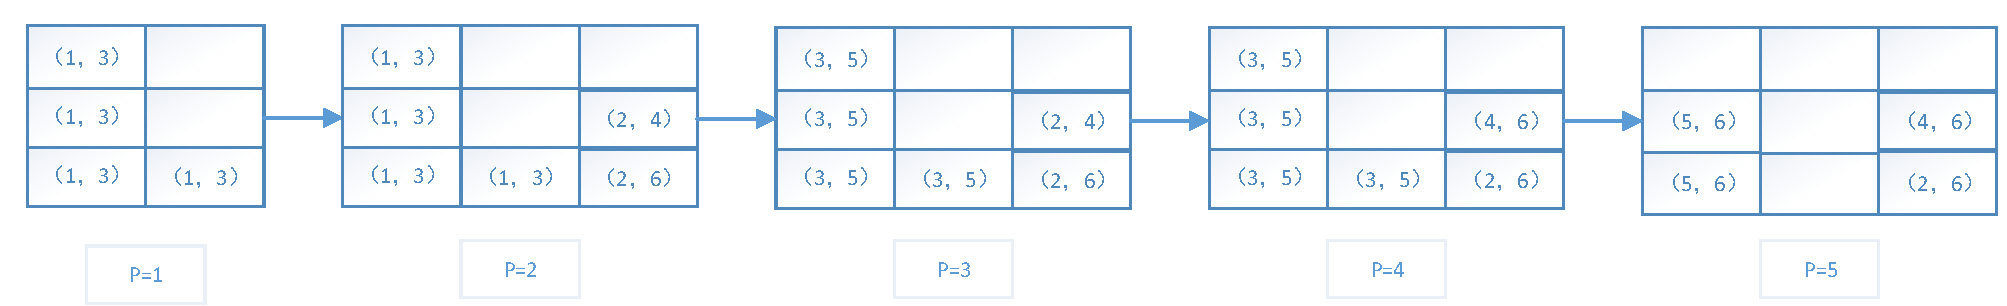
\includegraphics{figure/without_rehandle.jpg}}
\label{fig 3:graph}
\end{figure}

If they are loaded with rehandles, the loading sequence and layout will be the following Figure \ref{fig 4:graph}.
\begin{figure}[htbp]
\centering
\caption{stowage plan with rehandle.}
\resizebox{0.9\textwidth}{!}{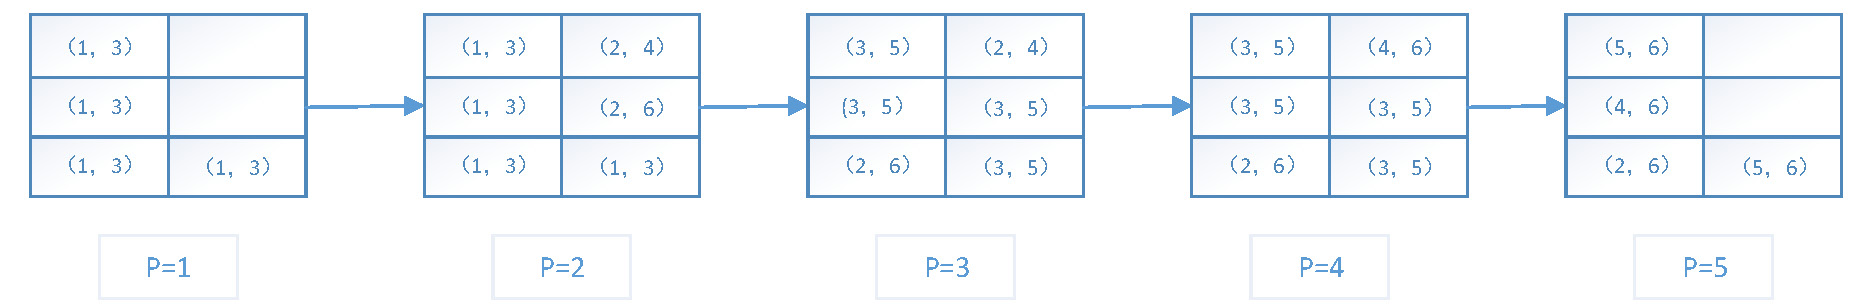
\includegraphics{figure/with_rehandle.jpg}}
\label{fig 4:graph}
\end{figure}

From the above figures, we can draw the conclusion that allowing a certain number of rehandles will reduce the number
of stacks used to store containers in a vessel compared with zero rehandle.
That's to say, the utilization of containership can be improved if some rehandles are allowed.

We also use some pictures to make our results more visual and the pictures are made by Excel.

\begin{figure}[htbp]
\center
\caption{Relationship between allowed rehandle and used stacks}
\resizebox{0.5\textwidth}{!}{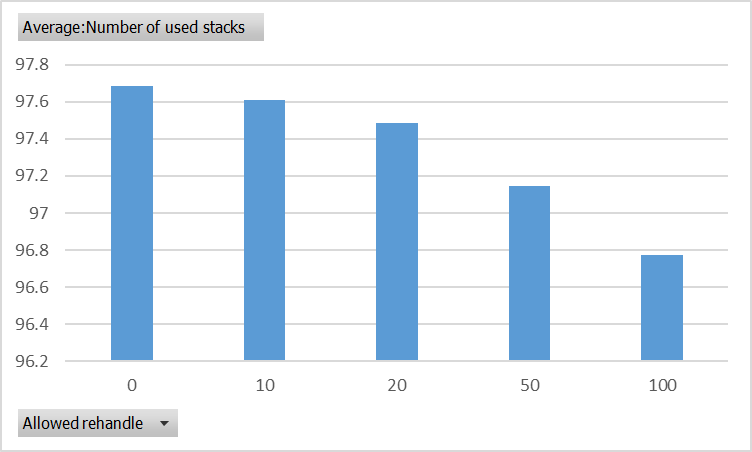
\includegraphics{figure/K-Stacks.png}}
\label{fig 5:graph}
\end{figure}
As what is shown in Table \ref{tab:4}, Figure \ref{fig 5:graph} indicates visually the relationship between used stacks and allowed rehandle.
It's not hard to draw the conclusion that the more allowed rehandle, the less used stacks.
So it intuitively reflects the meaning of this research and it shows the feasibility of our algorithm.
Comparing with zero rehandle, some rehandles are allowed to reduce the partial stacks and improve the utilization of containership.

\begin{figure}[htbp]
\centering
\caption{Relationship between containers and used stacks}
\resizebox{0.5\textwidth}{!}{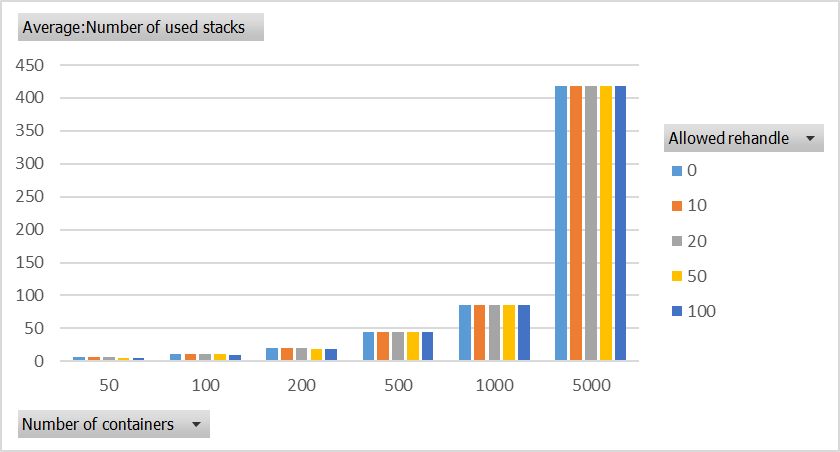
\includegraphics{figure/K-containers.png}}
\label{fig 6:graph}
\end{figure}
Figure \ref{fig 6:graph} shows us the relationship between containers and used stacks.
We can conclude that the more containers are, the more stacks will be used, which is undoubted in practice.
Another conclusion can be drawn is that the more containers, the difference caused by rehandles is less.


\begin{figure}[htbp]
\centering
\caption{Relationship between ports and used stacks}
\resizebox{0.5\textwidth}{!}{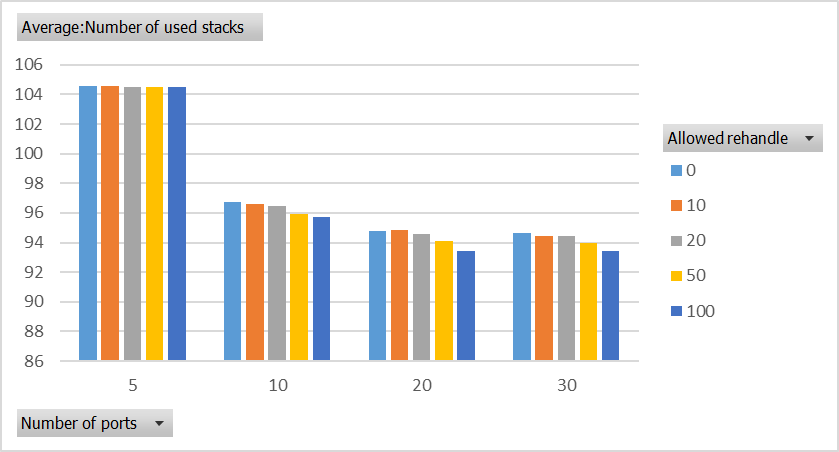
\includegraphics{figure/K-ports.png}}
\label{fig 7:graph}
\end{figure}
Figure \ref{fig 7:graph} provides us the relationship between ports and used stack. In general, the more ports are among the shipping, the more stacks will be used.
Another related factor to be  taken into consideration is the sparse distribution situation of containers in each port.

\begin{figure}[htbp]
\centering
\caption{Relationship between limit height and used stacks}
\resizebox{0.5\textwidth}{!}{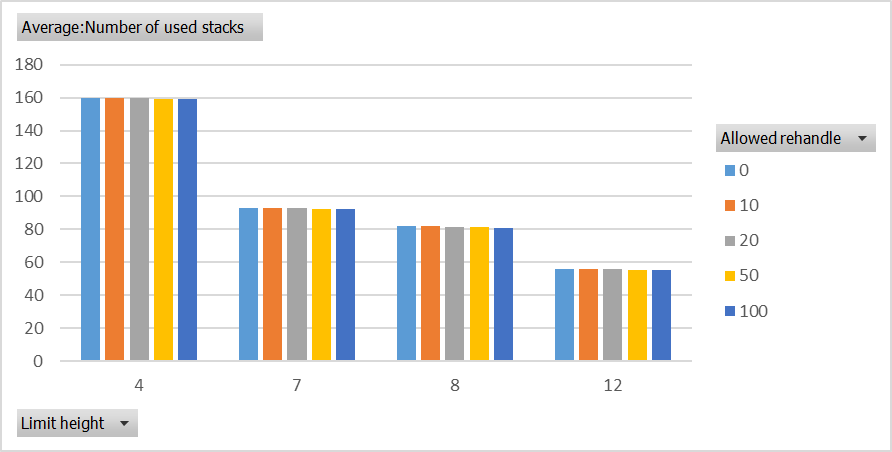
\includegraphics{figure/K-limit_height.png}}
\label{fig 8:graph}
\end{figure}
Figure \ref{fig 8:graph} shows us that the larger the number of limit height is, the less stacks will be used, which is definitely right.


\begin{figure}
\centering
\caption{Relationship between comprehensive factors and used stacks}
\resizebox{0.5\textwidth}{!}{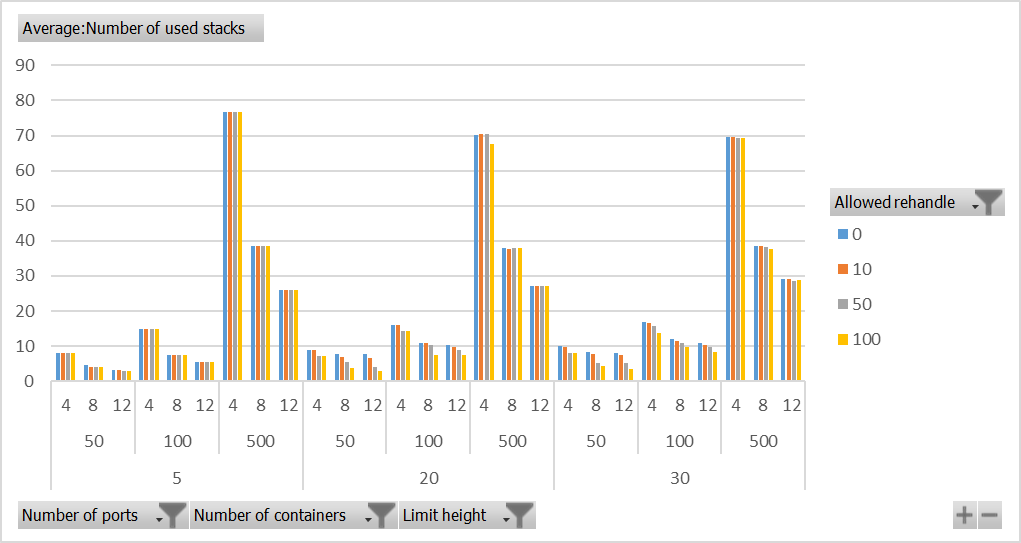
\includegraphics{figure/K-comprehensive.png}}
\label{fig 9:graph}
\end{figure}
Figure \ref{fig 9:graph} shows us that the comprehensive impact on the result we work out with all the basic factors considered in this paper.
Further, we can choose the factors we want to analyze one by one and it is convenient for us to work out how different factors influence our final result.
For the convenience of observation, we only give the result with filtered numbers of each factor.


\section{Conclusion}
\label{sec:con}
The stowage stack minimization problem with K-rehandle constraint (SSMP-KR) is aimed to find out a stowage plan that fewest stacks on a containership are required to accommodate given containers throughout a voyage by subject to K-rehandles.

In this paper, we analyze the structure of this two-dimensional bin-packing optimization problem and its relationship with the SSMP-ZR problem proposed in \cite{wang2014stowage}.

We can regard the stowage stack minimization problem with zero rehandle as an particular case when we choose the value of K as zero.
Hence, the problem proposed in this paper is a generalized and extended problem of SSMP-ZR considering the existence of K-rehandle.

On the one hand, the stowage planning problems in cyclic navigation path is converted into linear navigation path using the specific method.
On the other hand, the result is equivalent to each other whether we convert or not.

In this paper, we presented the integer programming model for the SSMP-ZR and presented a simple IP model for the SSMP-KR.

A heuristic approach is proposed to construct near-optimal solutions to the SSMP-KR problem in a very short computational time.
Since there are different status in the process of handling containers, different methods in our algorithm are thought to cope with the corresponding conditions.

The experimental results show that our heuristic approaches generate very promising solutions on a variety of instances.
Comparing with the stowage stack minimum problem with zero constraint, our problem with K rehandle constraint can offer a certain flexibility for the actual problem.
The results show the problem we put forward is of practical significance and it can improve the utilization of containership.
Our algorithm uses greedy rules to find the best slot for each container, hence the results may be the near-optimal rather than global optimal.
As we all know, it is difficult to get the global optimal for this kind of problem.
Applying this algorithm into the real shipping management can enhance the hull space utilization and reduce some spending in the case of improving the utilization of containership.
The novelty and practicality show the importance of this paper and it can give a reference to the future study.


Furthermore, the rehandles are unavoidable in the actual port operation, which indicates the problem we propose in this paper does make some
sense and the solution we work out using our heuristic algorithm can provide a preliminary assessment for forwarders to arrange
linear shipping company for transportation.


\bibliographystyle{apalike2}
\bibliography{references}
\end{document}


